\setlength\dashlinedash{0.2pt}
\setlength\dashlinegap{1.5pt}
\setlength\arrayrulewidth{0.3pt}

\begin{table*}[t]
\small
\begin{adjustbox}{width=1.0\textwidth}
\begin{tabular}{lllllllllllll}
\toprule
\multirow{3}{*}{\textbf{Model}} & \multicolumn{6}{c}{\attribute{profession}} & \multicolumn{6}{c}{\attribute{hobby}} \\
\cmidrule(lr){2-7} \cmidrule(lr){8-13}
  &  \multicolumn{2}{c}{\wiki{page}}  &  \multicolumn{2}{c}{\wiki{category}}  &  \multicolumn{2}{c}{Web search}  &  \multicolumn{2}{c}{\wiki{page}}  &  \multicolumn{2}{c}{\wiki{category}}  &  \multicolumn{2}{c}{Web search}   \\
\cmidrule(lr){2-3} \cmidrule(lr){4-5} \cmidrule(lr){6-7} \cmidrule(lr){8-9} \cmidrule(lr){10-11} \cmidrule(lr){12-13}
  &  \textsc{mrr}  &  n\textsc{dcg}  &  \textsc{mrr}  &  n\textsc{dcg}  &  \textsc{mrr}  &  n\textsc{dcg}  &  \textsc{mrr}  &  n\textsc{dcg}  &  \textsc{mrr}  &  n\textsc{dcg}  &  \textsc{mrr}  &  n\textsc{dcg}  \\
\midrule
No-keyword + BM25  &  .15*  &  .32*  &  .17*  &  .37*  &  .11*  &  .28*  &  .16*  &  .42*  &  .13*  &  .35*  &  .06*  &  .22*  \\
RAKE + BM25        &  .16*  &  .33*  &  .19*  &  .39*  &  .11*  &  .28*  &  .17*  &  .42*  &  .14*  &  .37*  &  .07*  &  .23*  \\
RAKE + KNRM        &  .16*  &  .33*  &  .13*  &  .34*  &  .15*  &  .34*  &  .12*  &  .32*  &  .12*  &  .31*  &  .06*  &  .24*  \\
TextRank + BM25    &  .21*  &  .39*  &  .26*  &  .45*  &  .15*  &  .32*  &  .21   &  .46   &  .20*  &  .42*  &  .10*  &  .28*  \\
TextRank + KNRM    &  .21*  &  .38*  &  .18*  &  .36*  &  .20*  &  .40*  &  .15*   &  .36*   &  .16*  &  .36*  &  .11*  &  .31*  \\
BERT IR    &  \best{.30}  &  .45  &  .28*  &  .44*  &  .26*  &  .38*  &  .22   &  .43*   &  .18*  & .42*    &  .15*  &  .33*  \\
\midrule
\charm{BM25}       &  .29   &  \best{.46}   &  .28*  &  .47*  &  .28*  &  .45*  &  \best{.24}   &  \best{.47}   &  .21*  &  .43*  &  .11*  &  .30*  \\
\charm{KNRM}       &  .27   &  .44   &  \best{.35}   &  \best{.55}   &  \best{.41}   &  \best{.59}   &  .22   &  .44*  &  \best{.27}   &  \best{.49}   &  \best{.19}   &  \best{.38}   \\
\bottomrule
\end{tabular}
\end{adjustbox}
\caption[Results for \emph{unseen} values for \textit{hobby} and \textit{profession}.]{Results for \emph{unseen} values.
Results marked with * significantly differ from the best method (in bold) measured by a paired t-test ($p<0.05$). As described in the experimental setup, BERT IR on Wiki-category and Web search must consider a subset of documents.
}
\label{tab3}
\end{table*}
\begin{table}[t] 
\small
\centering
\begin{adjustbox}{width=0.6\textwidth}
\begin{tabular}{llllll}
\toprule
\multirow{2}{*}{Model}  &  Document  &  \multicolumn{2}{c}{\attribute{profession}}  &  \multicolumn{2}{c}{\attribute{hobby}}  \\
\cmidrule(lr){3-4} \cmidrule(lr){5-6}
  &  collection  &  \textsc{mrr}  &  n\textsc{dcg}  &  \textsc{mrr}  &  n\textsc{dcg}  \\  
\midrule
N-GrAM          &  -                &  .13*  &  .43*  &  .11*  &  .40*  \\
W2V-C           &  -                &  .09*  &  .39*  &  .08*  &  .32*  \\
CNN             &  -                &  .20*  &  .52*  &  .14*  &  .43*  \\
\method{2attn}  &  -                &  .32*  &  .59*  &  .33   &  \best{.55}   \\
BERT            &  -                &  \best{.50}  &  \best{.68}  &  \best{.35}   &  \best{.55}   \\
\midrule
\charm{BM25}    &  \wiki{page}      &  .42*  &  .57*  &  .31*   &  .51*   \\
                &  \wiki{category}  &  .38*  &  .56*  &  .32   &  .50*  \\
                &  Web search       &  .49   &  .65   &  .31*  &  .51   \\
\midrule                
\charm{KNRM}    &  \wiki{page}      &  .37*  &  .54*  &  .28*  &  .46*  \\
                &  \wiki{category}  &  .43*  &  .62*  &  .31   &  .51*  \\
                &  Web search       &  .49   &  .66   &  .31   &  .51   \\
\bottomrule            
\end{tabular}
\end{adjustbox}
\caption[Results for \emph{seen} values for \textit{hobby} and \textit{profession}.]{Results for \emph{seen} values.
Results marked with * significantly differ from the best method (in bold face) measured by a paired t-test ($p<0.05$).
}
\label{tab4}
\end{table}

\subsection{Quantitative Results}

\paragraphHdTop{\emph{Unseen} values (zero-shot mode).}
The models' performance evaluated only on the attribute values that were not observed during training is shown in Table \ref{tab3}.
Both CHARM variants significantly outperform all unsupervised keyword-extraction baselines for both attributes on all document collections. This suggests the importance of training the cue detector to identify terms related to the attribute, instead of the more general keywords usually given by unsupervised keyword extractors.
BERT IR performs similarly to CHARM for the \wiki{page} dataset, but shows significantly worse results for the remaining datasets, taking approximately 60x longer than \charm{KNRM} to perform inference.

Interestingly, the \emph{No-keyword} method performs on par with the other baselines. It shows that the words produced by the state-of-the-art keyword extraction models are not more helpful than the ones automatically selected by TF-IDF scores in BM25 model, highlighting the difficulty of keyword extraction from conversational data.

For both attributes, \charm{KNRM} always outperforms the BM25 variant on \wiki{category} and Web search collections. This may be related to the size of document collections, which allows for more variations in the vocabularies that are captured well by the term embeddings in KNRM. Another observation is that for \charm{KNRM}, while Web search yields the best result for \emph{profession}, \wiki{category} is the best collection for \emph{hobby}, possibly due to the noisy hobby-related documents from web search.
\charm{BM25} on \wiki{page} does not require any additional inputs and consistently performs as well as or better than the baselines across both attributes. 
\wiki{category} performs significantly better than all baselines for both attributes, making it a reasonable choice when Wikipedia categories are available.

To demonstrate that the collections are resilient to inaccuracies in their automatic construction, we conducted an experiment where some percentage of the documents' attribute values were randomly changed. We found that randomly changing 20\% of the documents' labels resulted in approximately a 15\% MRR decrease for \charm{KNRM} on Web-search and Wiki-category.
The performance decrease on these collections was roughly linear.
This indicates that the noise in the document collection does not severely damage CHARM's performance.

\paragraphHd{\emph{Seen} values (supervised mode).}
In this experiment we evaluate CHARM's performance in the fully supervised setting (i.e., all labels are seen during training).
From the Table \ref{tab4} we observe that CHARM's performance is competitive compared to \method{2attn} (i.e., the best-performing attribute value prediction method from prior work) and the state-of-the-art BERT model.
The fully supervised BERT model consistently performs best for both attributes, though these increases are not statistically significant over all CHARM configurations. Furthermore, BERT and \method{2attn} are trained with full supervision in this experimental setting, whereas CHARM still uses a policy gradient.

Another observation is that in this experiment the Web search collection consistently performs best, suggesting that the collection's shortcomings are mitigated when all labels are observed.


\balance
\subsection{Qualitative Analysis}

\paragraphHd{Analysis of selected terms}
For each attribute value, we gathered all query terms for the users predicted as having this attribute value, together with the term scores from the cue detector.
We then averaged the scores for each term within an attribute value, and selected top 10 terms as the representative ones. 
Terms were extracted using \charm{KNRM} on \wiki{category} in \emph{unseen} experiments.
We performed the same method for the TextRank keywords, because this was the best performing keyword-based baseline in the \emph{unseen} experiments.
The comparison of selected terms by CHARM vs TextRank is reported in Table \ref{tab:top_terms} and Table \ref{tab:top_words} for selected attribute values of \emph{profession} and \emph{hobby} respectively.


\begin{table}[h!]
\vspace{10pt}
    \centering
    \footnotesize
    \begin{adjustbox}{width=0.8\textwidth}
    \begin{tabular}{ll@{}rl@{}rl@{}r}
\toprule
                          & \multicolumn{6}{c}{\attribute{profession}}   \\
\cmidrule(lr){2-7} 
                          & \multicolumn{2}{c}{\textbf{barista}}      & \multicolumn{2}{c}{\textbf{screenwriter}} & \multicolumn{2}{c}{\textbf{airplane pilot}}  \\
                          & \multicolumn{2}{c}{(MRR=0.4,}    & \multicolumn{2}{c}{(MRR=0.65,}   & \multicolumn{2}{c}{(MRR=0.64,}     \\
                          & \multicolumn{2}{c}{\#sample=73)} & \multicolumn{2}{c}{\#sample=52)} & \multicolumn{2}{c}{\#sample=14)}   \\ \midrule
\multirow{5}{*}{CHARM}    & coffee           & shop           & script        & story            & pilot            & flying            \\
                          & starbucks        & guitar         & screenplay    & film    & flight           & teacher           \\
                          & store            & student        & screenwriting & films            & training         & fire              \\
                          & school           & customer       & scripts       & photo            & fly              & trading           \\
                          & manager          & college        & writing       & movie            & pilots           & military          \\ \midrule
\multirow{5}{*}{TextRank} & people           & amp            & first         & hollywood        & people           & american          \\
                          & first            & love           & people        & tomorrow         & first            & lots              \\
                          & coffee           & things         & thanks        & time             & things           & guy               \\
                          & today            & starbucks      & amp           & second           & today            & time              \\
                          & thanks           & work           & stuff         & one              & thanks           & guys              \\ \bottomrule
\end{tabular}
    \end{adjustbox}
    \caption{\charm{KNRM}'s top 10 terms per label for \emph{profession} attribute, compared with TextRank keywords.}
\vspace{7pt}
    \label{tab:top_terms}
\end{table}

We can observe that regardless of the small sample size for some values like \textit{airplane pilot}, CHARM can still detect meaningful words. For \textit{barista}, CHARM did not even consider the term `barista', but rather focused on the words such as `coffee' and `starbucks'. 
Choosing terms like `screenplay', `scripts' and `screenwriting' helps the model to distinguish \textit{screenwriter} from the other film-related professions like \emph{director}.

Picking the terms like `cake', `baking' and `bread', helps the model to distinguish between \textit{baking} and \textit{cooking} hobbies more effectively.
Note, that even for rare unusual hobbies like \textit{quilting}, CHARM manages to select indicative terms. This essentially shows that the model can easily be used for large long-tailed lists of attribute values.

For the attribute values where CHARM's MRR scores are considerably high (e.g., \emph{profession:screenwriter}, \emph{hobby:baking}), the detected cues are meaningful, diverse and quite distinctive. 
On the other hand, for attribute values with low MRR scores, some terms are representative, however, they are also easily confused with other attribute values. For instance, some \emph{model aircraft} hobby terms  may also refer to the \emph{air sports} hobby.

Finally, as opposed to CHARM, TextRank keywords rarely make sense. This suggests that unsupervised keyword detectors are not capable of producing useful attribute-value-related keywords from users' utterances. 


\begin{table}[ht!]
\vspace{10pt}
    \centering
    \footnotesize
    \begin{adjustbox}{width=0.8\textwidth}
    \begin{tabular}{llrlrlr}
\toprule
                          & \multicolumn{6}{c}{\attribute{hobby}}                                                                                 \\
\cmidrule(lr){2-7} 
                          & \multicolumn{2}{c}{\textbf{baking}}       & \multicolumn{2}{c}{\textbf{quilting}}     & \multicolumn{2}{c}{\textbf{model aircraft}} \\
                          & \multicolumn{2}{c}{(MRR=0.46,}   & \multicolumn{2}{c}{(MRR=0.26,}   & \multicolumn{2}{c}{(MRR=0.11,}     \\
                          & \multicolumn{2}{c}{\#sample=64)} & \multicolumn{2}{c}{\#sample=27)} & \multicolumn{2}{c}{\#sample=2)}    \\ \midrule
\multirow{5}{*}{CHARM}    & cake            & bread           & sewing          & way            & cat               & dimensions      \\
                          & food            & cream           & quilting        & game           & plane             & pilots          \\
                          & recipe          & cooking         & quilt           & metal          & construction      & song            \\
                          & cheese          & pasta           & fabric          & design         & planes            & steam           \\
                          & baking          & cook            & music           & playing        & energy            & music           \\ \midrule
\multirow{5}{*}{TextRank} & thanks          & things          & thanks          & today          & thanks            & work            \\
                          & first           & work            & first           & science        & german            & elyrion         \\
                          & amp             & food            & things          & kids           & steam             & time            \\
                          & people          & time            & people          & time           & tapjoy            & purchase        \\
                          & recipes         & second          & amp             & lots           & motorola          & air             \\ \bottomrule
\end{tabular}
    \end{adjustbox}
    \caption{\charm{KNRM}'s top 10 terms per label for \emph{hobby} attribute, compared with TextRank keywords.}
\vspace{7pt}
    \label{tab:top_words}
\end{table}

\paragraphHd{Misclassification Study}
To conduct error analysis, we plotted a confusion matrix of \charm{KNRM} in the \emph{unseen} experiment for \emph{profession} attribute, which is shown in Figure \ref{conf_prof}.

We observe that medical professions such as \textit{dentist, nurse, pharmacist} and \emph{surgeon} are often confused to \textit{doctor} in general. Professions associated with studying (\textit{academic, teacher} and \emph{student}), beauty (\textit{hairdresser} and \emph{tattoo artist}) and art (\textit{musician} and \textit{poet}) are often confused with each other. \textit{Salesman} and \emph{accountant} are confused to \textit{broker}, because of the common financial terms used. 

%Hobbies associated with music (\textit{dancing, singing} and \emph{music}) and images (\textit{painting}, \emph{graphic design} and \emph{photography}) are often mixed up. Hobbies in which the term `game' is profusely used like \textit{chess} and \emph{baseball} are confused to \textit{board games}; similarly, \textit{fishing} and \textit{fish keeping}, as well as \textit{skiing} and \emph{snowboarding} are confused due to the common lexicon used.

\begin{figure}[h!]
 \centering
   \centering
   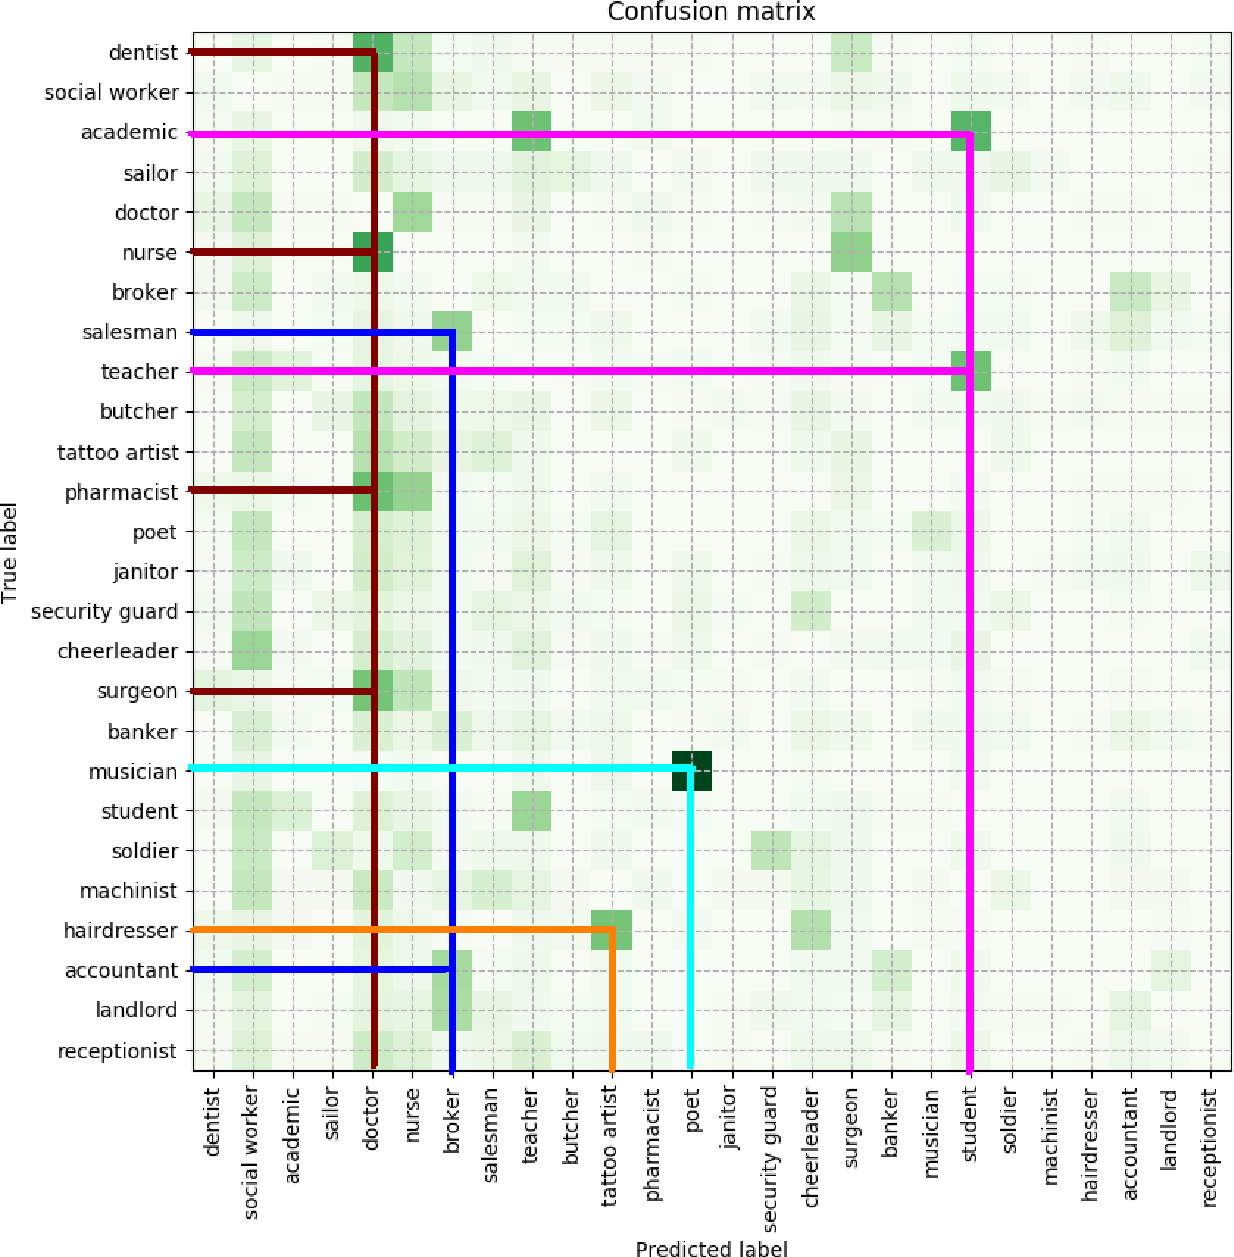
\includegraphics[scale=0.5]{imgs/profession_confusion.pdf}
\vspace{0.3cm}
\caption{Confusion matrix for \emph{profession}  with \charm{KNRM} on \emph{unseen} experiments, with some values removed for brevity. Unseen values are aggregated across folds. 
Darker cells indicate more misclassifications. The lines illustrate misclassifications of interest.
}
   \label{conf_prof}
\end{figure}

%\begin{figure*}[h!]
% \centering
% \begin{subfigure}{.49\textwidth}
%   \centering
%   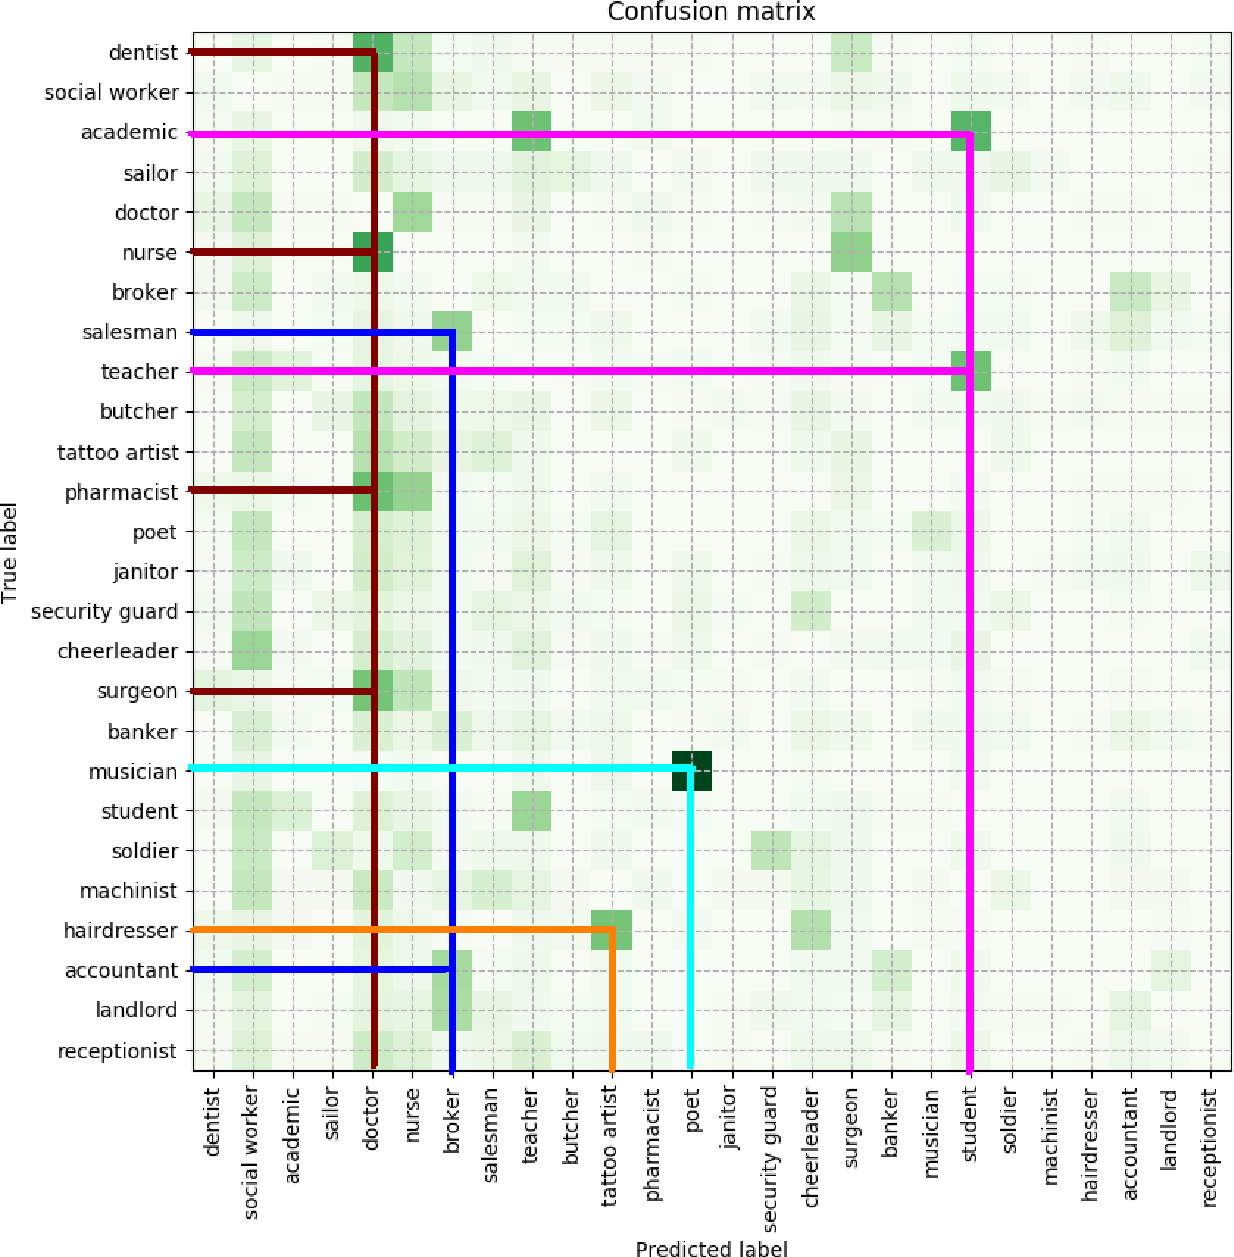
\includegraphics[scale=0.32]{imgs/profession_confusion.pdf}
%   \caption{\textit{profession}}
%   \label{conf_prof}
% \end{subfigure}
% \begin{subfigure}{.49\textwidth}
%   \centering
%   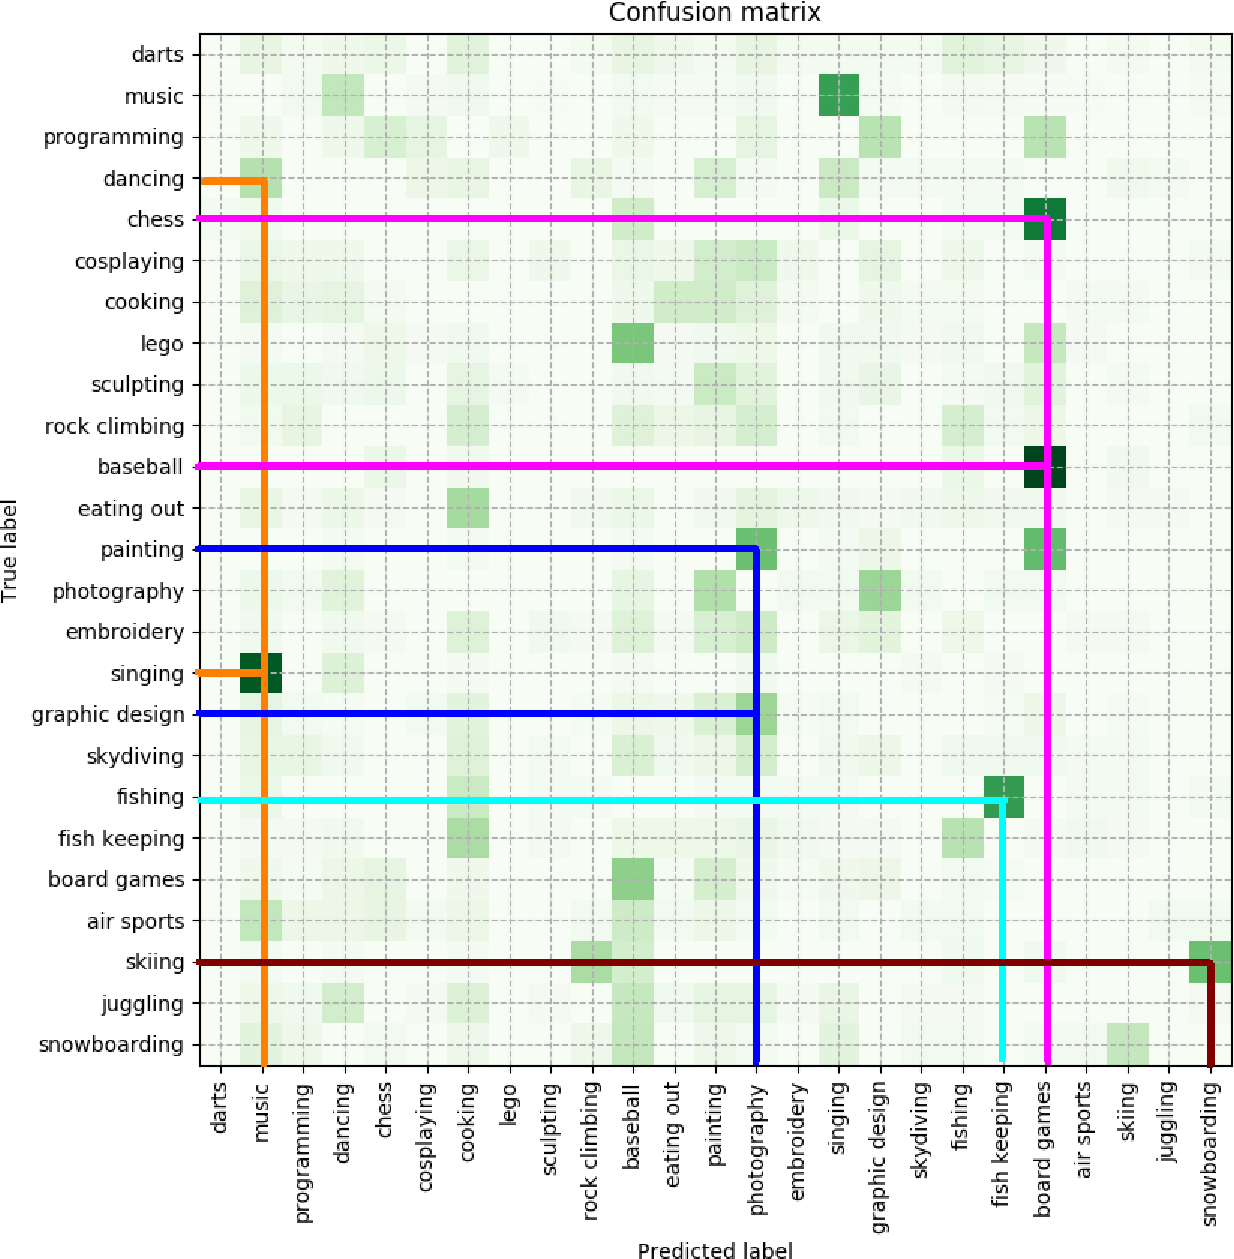
\includegraphics[scale=0.32]{imgs/hobby_confusion.pdf}
%   \caption{\textit{hobby}}
%   \label{conf_hob}
% \end{subfigure}
%\vspace*{-0.3cm}
%\caption{Confusion matrix for \emph{profession} and \emph{hobby} with \charm{KNRM} on \emph{unseen} experiments, with some values removed for brevity. Unseen values are aggregated across folds. 
%Darker cells indicate more misclassifications. The lines illustrate misclassifications of interest.
%}
%\label{fig:conf-profession-hobby}
%\end{figure*}


\paragraphHd{Analysis of top ranked documents}
For each attribute value, we collected all documents that were returned for a user with the given value as the ground-truth label. We then averaged the scores for each document and selected the top 5 retrieved documents from \wiki{category},
shown in Table \ref{tab:top_pages} for several \emph{profession} and \emph{hobby} attribute values.

It is interesting to observe that in spite of the common lexicon for some similar values, the model manages to retrieve documents which are relevant to a particular value, e.g., documents for \textit{investor}  are distinct from other financial-related professions, like \textit{broker} or \textit{salesman}.
It is also worth mentioning that the retrieved pages for \textit{investor} and \textit{ice hockey} are rather the pages for related lexicon (e.g., \textit{venture capital} and \textit{playoff beard} respectively), which shows the ability of CHARM to detect indirect cues.


\begin{table*}[t!]
    \centering
    \footnotesize
    \begin{adjustbox}{width=0.95\textwidth}
    \begin{tabular}{llll}
\toprule
                            \multicolumn{2}{c}{\attribute{profession}} & \multicolumn{2}{c}{\attribute{hobby}}                                                                                                                 \\
\cmidrule(lr){1-2} \cmidrule(lr){3-4}
                            \textbf{firefighter} (MRR=0.46)                & \textbf{investor} (MRR=0.52)                      & \textbf{knitting} (MRR=0.68)                                                & \textbf{ice hockey} (MRR=0.68)                         \\ \midrule
                            Firefighter                                          & Index\_fund                                       & Yarn\_over                                               & Extra\_attacker                                     \\
                            Firefighter\_assist\_and\_search\_team              & Venture\_capital                                  & Brioche\_knitting                                        & Ice\_hockey\_rules                                  \\
                            Calvert\_County\_Fire-Rescue-EMS                    & Treasury\_management                              & Combined\_knitting                                       & Neutral\_zone\_trap                                 \\
                            Firefighter\_arson                                  & Buy\_side                                         & Flat\_knitting                                          & Playoff\_beard                                      \\
                            Fire\_captain                                       & Sovereign\_wealth\_fund                           & Tunisian\_crochet                                        & Line\_(ice\_hockey)                                 \\  \bottomrule
\end{tabular}
    \end{adjustbox}
    \caption{\charm{KNRM}'s top 5 retrieved documents per attribute value.}
    \label{tab:top_pages}
\end{table*}